%
% ICRA 2013 Paper Submission
% created on Sep 5, 2012
%
\def \papertitle{Cooperative Control for Window Traversal with an Ornithopter Micro Air Vehicle and Lightweight Ground Station}

% NOTE: WE WRITE ALL TEXT IN FIRST PERSON PLURAL ("we")
% Conventions: flapping-wing, small-scale

%!TEX TS-program = latex
%!TEX encoding = UTF-8 Unicode

\documentclass[letterpaper, 10 pt, conference]{ieeeconf}
\IEEEoverridecommandlockouts % for \thanks
\overrideIEEEmargins % for \addtolength

% Packages
\usepackage{color}
\usepackage[pdftex]{graphicx}
\usepackage{subfig}
\usepackage{multirow}
\usepackage{rotating}
\usepackage[pdftex]{hyperref}

% hyperref setup
\definecolor{linkCol}{gray}{0.25}
\hypersetup{
    pdftitle={\papertitle},
    pdfauthor={Ryan C. Julian, Cameron J. Rose, Humphrey Hu, and Ronald S. Fearing},
    pdfsubject={},
    pdfkeywords={},
    pdfpagemode=UseOutlines, bookmarksopen, bookmarksnumbered,
    colorlinks, linkcolor=linkCol, citecolor=linkCol, urlcolor=linkCol
}

% Title
\title{\LARGE \bf \papertitle}

% Authors
\author{
    Ryan C. Julian$^{*}$,
    Cameron J. Rose$^{*}$,
    Humphrey Hu$^{\dagger}$, and
    Ronald S. Fearing$^{*}$
    \thanks{$^{*}$
    	R.C. Julian, C.J. Rose and R.S. Fearing are
        with the Department of Electrical Engineering and Computer Sciences,
        University of California, Berkeley, CA 94720 USA.
        \href{mailto:ryanjulian@berkeley.edu}{\tt ryanjulian@berkeley.edu},
        \href{mailto:c\_rose@eecs.berkeley.edu}{\tt c\_rose@eecs.berkeley.edu},
        \href{mailto:ronf@eecs.berkeley.edu}{\tt ronf@eecs.berkeley.edu}
    }
    \thanks{$^{\dagger}$
        H. Hu is with the Robotics Institute,
        Carnegie Mellon University, Pittsburgh, PA 15213 USA.
        \href{mailto:humphreh@andrew.cmu.edu}{\tt humphreh@andrew.cmu.edu}
    }
    \thanks{
        This material is based upon work supported by the National Science
        Foundation under Grants No. CNS-0931463, and by the Army Research
        Laboratory under the Micro Autonomous System and Technology
        Collaborative Technology Alliance.
    }
}

\begin{document}

\maketitle
\thispagestyle{empty}
\pagestyle{empty}

%%%%%%%%%%%%%%%%%%%%%%%%%%%%%%%%%%%%%%%%%%%%%%%%%%%%%%%%%%%%%%%%%%%%%%%%%%%%%%
\begin{abstract}
The power, size, and weight constraints of micro air vehicle (MAV) platforms limit their on-board sensing and computational resources. Ground vehicles have less mobility than MAVs, but relaxed size constrains and typically more computing power, creating a opportunity for cooperation between the two platforms. In this work, we demonstrate cooperative target-seeking by a 14 gram ornithopter MAV with a lightweight ground station using computer vision. We also introduce a new ornithopter MAV platform, the H$^2$Bird, which features clap and fling flight mechanics and improves upon a previous design with yaw and pitch control and improved payload. To augment the built-in navigation and sensing capabilities of the ornithopter, the ground station to provides heading estimates to the ornithoper by running a real-time motion tracking algorithm over the a live video stream. This allows the ornithopter to negotiate indoor navigation through a window. We discuss the performance of both the location estimation and navigation algorithms. We analytically determine the backwards-reachable region for successfully navigating through the window, and use it to determine the operational limits of the system. Finally, we verify this region through data collected in experimental trials. We achieve a success rate of X\% within the feasible region.
\end{abstract}

%%%%%%%%%%%%%%%%%%%%%%%%%%%%%%%%%%%%%%%%%%%%%%%%%%%%%%%%%%%%%%%%%%%%%%%%%%%%%%
\section{Introduction}
%TODO(ryan)
The power, size, and weight constraints of micro air vehicle (MAV) platforms significantly limit on-board sensing and computational resources, and thus the complexity of the control and state estimation algorithms which can be executed on-board. These constraints are particularly severe for flapping wing MAVs offer the promise of superior safety, efficiency, and noise profile to rotor craft MAVs, but at the expense of payload weight.

%%%%%%%%%%%%%%%%%%%%%%%%%%%%%%%%%%%%%%%%%%%%%%%%%%%%%%%%%%%%%%%%%%%%%%%%%%%%%%
\section{Robotic and Vision Platforms}
%TODO(ryan)

%----------------------------------------------------------------------------%
\subsection{H$^2$Bird Ornithoper MAV}
%TODO(humphrey)

\begin{figure}[tb]
\centering
\includegraphics[width=\linewidth]{figures/h2bird.png}
\caption{H$^2$Bird Ornithopter MAV}
\label{fig:h2bird}
\end{figure}

The flying platform used in this experiment is the H$^2$Bird flapping wing MAV. Built around the Silverlit I-Bird RC flyer powertrain and clap-fling wings, the H$^2$Bird has a wingspan of [40?] cm and weighs [14?] grams fully loaded. A tail propeller and servo-controlled tail elevator provide control in the yaw and pitch axes. An onboard electronics package combines a 40 MIPS microprocessor, 6 DOF IMU, 802.15.4 radio, VGA camera, and motor drivers with a 90 mAh lithium polymer battery for autonomous flight. In routine flight, the H$^2$Bird averages [insert speed] m/s ground speed and can operate for approximately [10] minutes.

%----------------------------------------------------------------------------%
\subsection{Ground Station Computer Vision Platform}
%TODO(ryan)

%%%%%%%%%%%%%%%%%%%%%%%%%%%%%%%%%%%%%%%%%%%%%%%%%%%%%%%%%%%%%%%%%%%%%%%%%%%%%%

%%%%%%%%%%%%%%%%%%%%%%%%%%%%%%%%%%%%%%%%%%%%%%%%%%%%%%%%%%%%%%%%%%%%%%%%%%%%%%
\section{System Concept and Algorithms}
%TODO(ryan)

\begin{figure}[tb]
\centering
\includegraphics[width=\linewidth]{figures/process_flow.pdf}
\caption{Process flow diagram for the cooperative control system.}
\label{fig:process_flow}
\end{figure}

%----------------------------------------------------------------------------%
\subsection{Ornithoper Flight Control}
%TODO(humphrey)

\begin{figure}[tb]
\centering
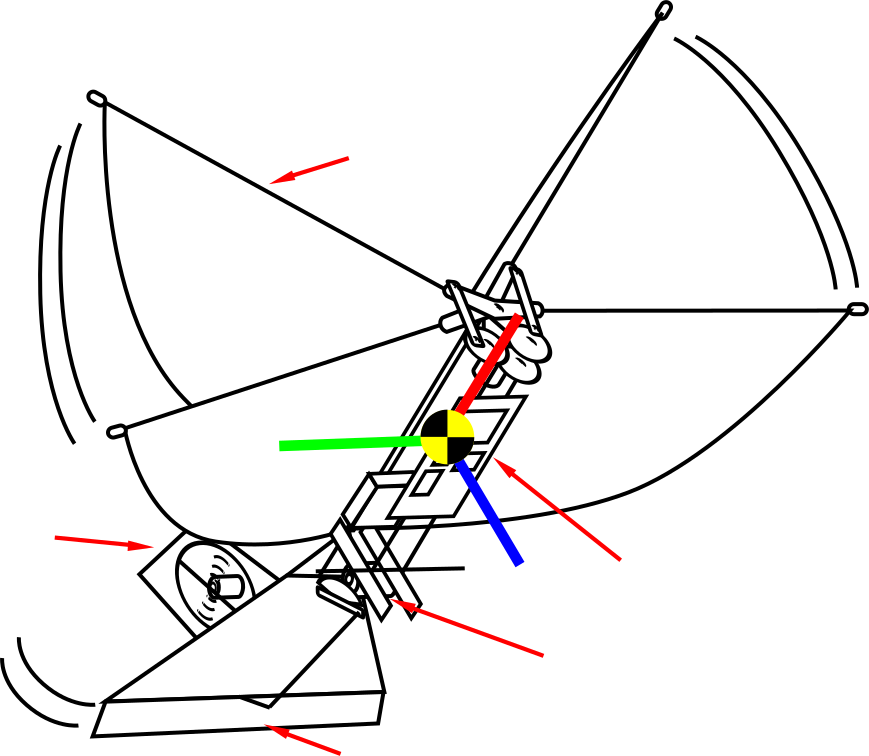
\includegraphics[width=\linewidth]{figures/h2bird_axes.jpg}
\caption{H$^2$Bird Ornithopter with flight control axes}
\label{fig:h2Bird_axes}
\end{figure}

Rudimentary attitude control for the H$^2$Bird runs on-board. It estimates pose by naively integrating the IMU and depending on PID for control. The simplistic nature of our state estimation and control is due to the stringent resource constraints applied by the platform.

We use simple controllers to actuate the H$^2$Bird's wing beat frequency, tail rotor, and tail elevator, which we designed to actuate thrust, yaw, and pitch respectively.

Due to the high pitch angles experienced by the H$^2$Bird, we use a quaternion representation of vehicle pose to avoid the numerical instabilities of Euler angle representations. This choice of pose representation also lends itself well to remote guidance, as relative body and world coordinate angular displacements can be represented compactly with quaternion multiplication.  

Given a reference pose $q$, we define the error $q_e$ as the rotation required to reach the reference pose from the measured pose. We then linearize the error quaternion to produce body axis angular errors as as inputs to the attitude controllers. 

Three independent proportional-integral-derivative controllers commanding the wing thrust, elevator, and tail propeller. We use this independent PID controller architecture for simplicity in tuning and implementation, and because it demonstrates acceptable performance in the absence of a system model.

\begin{equation}
\label{quat_error}
q_e = q'\otimes q_r
\end{equation}

\begin{equation}
\label{quat_angle}
\alpha = 2acos(q_{e,w})
\end{equation}

\begin{equation}
\label{quat_linearize}
Q_e = \alpha*q_e/sin(\alpha /2)
\end{equation}

%----------------------------------------------------------------------------%
\subsection{Pose Estimation}
%TODO(ryan)

%----------------------------------------------------------------------------%
\subsection{Visual Servoing}
%TODO(ryan)

\begin{figure}[tb]
\centering
\includegraphics[width=\linewidth]{figures/block_diagrams.pdf}
\caption{Overall block diagram of cooperative control}
\label{fig:block_diagram}
\end{figure}

\begin{figure}[tb]
\centering
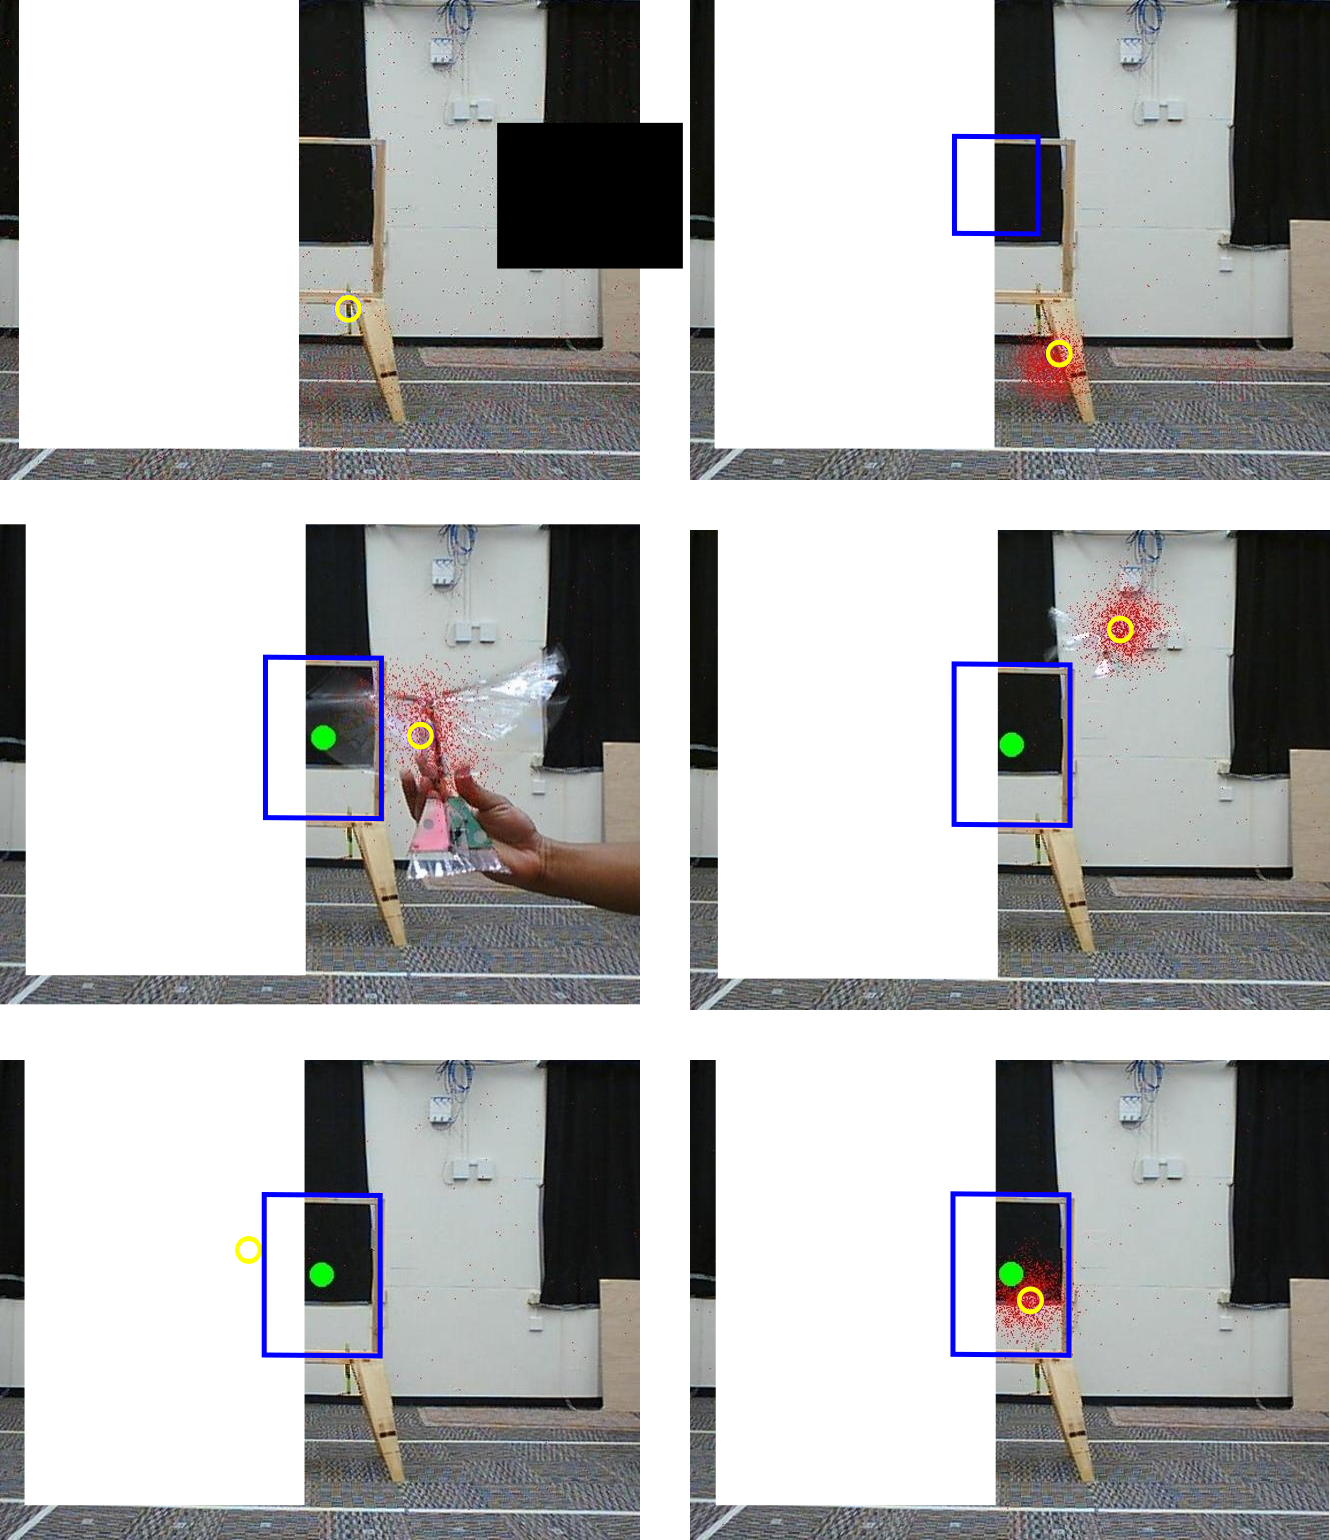
\includegraphics[width=\linewidth]{figures/pf_screencap.pdf}
\caption{Frame sequence from video feed used for tracking, showing particles and state estimate}
\label{fig:pf_screencap}
\end{figure}



%%%%%%%%%%%%%%%%%%%%%%%%%%%%%%%%%%%%%%%%%%%%%%%%%%%%%%%%%%%%%%%%%%%%%%%%%%%%%%

%%%%%%%%%%%%%%%%%%%%%%%%%%%%%%%%%%%%%%%%%%%%%%%%%%%%%%%%%%%%%%%%%%%%%%%%%%%%%%
\section{Experiments}
%TODO(ryan)

\begin{figure}[tb]
\centering
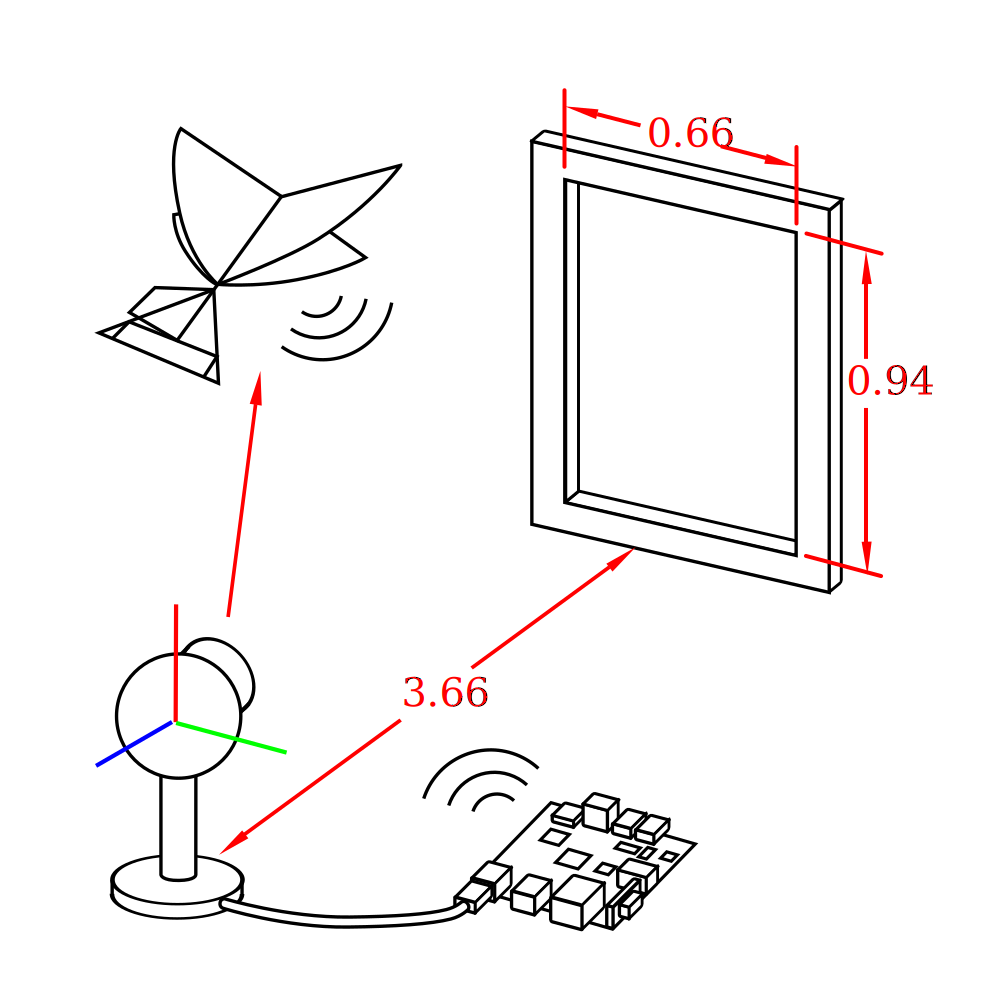
\includegraphics[width=\linewidth]{figures/experiment_cartoon.png}
\caption{Conceptual sketch of experimental environment.}
\label{fig:experiment_sketch}
\end{figure}

%%%%%%%%%%%%%%%%%%%%%%%%%%%%%%%%%%%%%%%%%%%%%%%%%%%%%%%%%%%%%%%%%%%%%%%%%%%%%%

%%%%%%%%%%%%%%%%%%%%%%%%%%%%%%%%%%%%%%%%%%%%%%%%%%%%%%%%%%%%%%%%%%%%%%%%%%%%%%
\section{Performance}
%TODO(ryan)

%----------------------------------------------------------------------------%
\subsection{Ornithopter Flight Control}
%TODO(cameron)
\begin{figure}[tb]
\centering
\includegraphics[width=\linewidth]{figures/step_response_total.pdf}
\caption{H$^2$Bird step response}
\label{fig:step_response}
\end{figure}

%----------------------------------------------------------------------------%
\subsection{Visual Servoing}
%TODO(ryan)

\begin{figure}[tb]
\centering
\includegraphics[width=\linewidth]{figures/flight_paths.pdf}
\caption{Plot of camera field-of-view and H$^2$Bird minimum turning radius cone, with experimental trials overlayed.}
\label{fig:flight_paths}
\end{figure}

%%%%%%%%%%%%%%%%%%%%%%%%%%%%%%%%%%%%%%%%%%%%%%%%%%%%%%%%%%%%%%%%%%%%%%%%%%%%%%
\addtolength{\textheight}{-0cm}
                        % This command serves to balance the column lengths
                        % on the last page of the document manually. It shortens
                        % the textheight of the last page by a suitable amount.
                        % This command does not take effect until the next page
                        % so it should come on the page before the last. Make
                        % sure that you do not shorten the textheight too much.


%%%%%%%%%%%%%%%%%%%%%%%%%%%%%%%%%%%%%%%%%%%%%%%%%%%%%%%%%%%%%%%%%%%%%%%%%%%%%%
\section{Conclusions and Future Work}
%TODO(ryan)

%%%%%%%%%%%%%%%%%%%%%%%%%%%%%%%%%%%%%%%%%%%%%%%%%%%%%%%%%%%%%%%%%%%%%%%%%%%%%%
\section{Acknowledgements}
The authors would like to thank Fernando Garcia Bermudez for his assistance with the Vicon motion capture system, Andrew Pullin for his help with robot photography, and the members of the Biomimetic Millisystems Laboratory and the EECS community at the University of California, Berkeley for their advice and support.
%%%%%%%%%%%%%%%%%%%%%%%%%%%%%%%%%%%%%%%%%%%%%%%%%%%%%%%%%%%%%%%%%%%%%%%%%%%%%%
\bibliographystyle{IEEEtranS}
\bibliography{}

\end{document}
